\subsection{Методы доступа к среде}
\label{sec:methods}

%Постоянно растущие требования пользователей к качеству обслуживания (QoS-требования) отражают изменения в структуре трафика в интернете. В частности, мультимедийный трафик (который производится такими приложениями, как VoIP, HD TV, видеоконференции и т.д.) занимает все больше и больше сетевых ресурсов. Поскольку ранние стандарты Wi-Fi поддерживали только  best effort transmissions, новые решения от Wi-Fi сообщества должны учитывать нужды пользователей.

%The constantly increasing users requirements for Quality of Service (QoS) reflect changes in the overall structure of the traffic in the Internet. In particular, multimedia traffic (generated by applications like VoIP, videoconferencing, High Definition TV, etc.) is occupying more and more network resources. QoS requirements of multimedia traffic include not only a minimal bandwidth but also a bounded delay and packet loss ratio. Since the early Wi-Fi standards were designed only for best effort transmissions, new solutions from the Wi-Fi community are requested to keep pace with the users needs. 

%As a response the IEEE 802.11 Working Group for WLAN Standards has produced the IEEE 802.11e amendment aimed to provide QoS support. 
%Particularly, the amendment introduced 
%The special attention paid to channel access methods is connected to a fact that in wireless networks the ability to provide QoS to a considerable degree depends on available channel access methods. Actually, in the last decade the IEEE 802.11 Working Group has made a number of steps in this direction. 

Дополнение IEEE 802.11e~\cite{802.11e} к стандарту Wi-Fi, направленное на внедрение поддержки QoS-требований, определило два новых механизма доступа: EDCA (Enhanced Distributed Channel Access) и HCCA (Hybrid coordination function Controlled Channel Access). Первый из них является механизмом приоритезированного случайного доступа к каналу, а второй -- механизмом детерминированного доступа.

С ростом плотности Wi-Fi-сетей HCCA и EDCA оказались не способны обеспечить надежную передачу данных, так как не обладают возможностями по работе в условиях жесткой интерференции. В частности, в случае большого числа точек доступа, работающих в одной области пространства, многие точки доступа выбирают один и тот же частотный канал. В результате EDCA страдает от множественных коллизий и эффекта скрытых станций. Ситуация с HCCA лишь немногим лучше за счет того, что HCCA исключает интерференцию со станциями своей сети. Поэтому возникает необходимость в разработке новых механизмов доступа, рассчитаных на работу в плотных сетях Wi-Fi.

Например, дополнение IEEE 802.11aa определяет механизм HCCA TXOP Negotiation, который позволяет точке доступа зарезервировать последовательность периодических интервалов времени, в течение которых она опрашивает свои станции, а соседние точки доступа (вместе со своими станциями) хранят молчание.  Данный подход существенно уменьшает интерференцию с соседними сетями, повышая надежность передачи. Стоит отметить, что интервалы времени резервируются не по одному, а целыми последовательностями: точка доступа резервирует \textit{последовательность периодических интервалов времени равной длительности}, в дальнейшем называемую \textit{периодическим резервированием}. Благодаря периодичности, все резервирование может быть описано с помощью всего лишь трех величин: \textit{периода} зерезервированных интервалов, их \textit{длительности} и \textit{момента начала первого интервала} (рис.~\ref{fig:periodic_reservation}).

\begin{figure}[h]
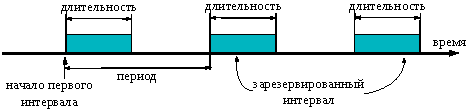
\includegraphics[width=\linewidth]{ReservedIntervals.pdf}
\caption{\label{fig:periodic_reservation} Периодическое резервирование}
\end{figure} 

%In wireless networks, the ability to provide QoS to a considerable degree depends on available channel access methods. That is why the first Wi-Fi amendment aimed for QoS support --- IEEE 802.11e~\cite{802.11e} --- has paid a special attention to this issue by defining two QoS-oriented channel access mechanisms: Enhanced Distributed Channel Access (EDCA) and Hybrid coordination function Controlled Channel Access (HCCA). The former is a \textit{random} (contention-based) channel access mechanism and provides prioritized QoS. The latter is an example of \textit{deterministic} channel access and provides parameterized QoS by means of contention-free polling.

%+ deterministic channel access schedule and other staff One of the key lying in the basis of reliable data transmission is deterministic channel access. Generally speaking, a deterministic channel access methods allow a station to preliminarily reserve a set of

%Дальнейшее развитие беспроводных технологий привело к появлению новых возможностей использования Wi-Fi в условиях высокой плотности сети. Высокая плотность сети подразумевает наличие большого числа точек доступа (AP) в одной области , that is, in Overlapping Basic Service Sets (OBSSs). Недостаток доступных для передачи частот заставляет соседние точки доступа передавать на одной и той же частоте. В случае использования EDCA в плотной сети эффективность этого механизма резко падает по причине существенной интерференции между станциями и частых коллизий. HCCA в состоянии лишь немного улучшить ситуацию, поскольку передача точки доступа, использующей HCCA, защищена только от пересечения с передачами станций (STA), ассоциированных с этой точкой доступа, но не с передачами других точек доступа. По этим причинам ни EDCA ни HCCA не могут предоставлять приемлемый уровень качества обслуживания в подобных ситуациях потому что они не предназначены для использования в сетях с высокой плотностью. Чтобы улучшить работу OBSS, дополнение IEEE 802.11aa, разработанное для робасной передачи аудио и видеопотоков добавило в HCCA the HCCA Negotiation procedure. Эта процедура позволяет точкам доступа резервировать интервалы времени, в течение которых точка доступа опрашивает свои станции, в то время как соседние точки доступа (вместе со своими станциями) не ведут передачу. Это и достигается за счет HCCA Negotiation, что подразумевает распространение точками доступа информации о зарезервированных интервалах. Данный подход существенно улучшает надежность передачи за счет дополнительных затрат. Для того чтобы уменьшить эти затраты, интервалы времени резервируются не по одному, а в рамках целой последовательности: точка доступа может резервировать \textit{последовательность периодически повторяющихся интервалов времени равной длительности}, что мы в дальнейшем будем называть \textit{периодическим резервированием}. Основная идея заключается в том, что всё резервирование может быть описано с помощью всего лишь трех величин: \textit{период} зерезервированных интервалов, их \textit{продолжительность} и \textit{момент начала первого интервала} (см рис.~\ref{fig:periodic_reservation}). 

%The further evolution of wireless technologies has leaded to the emergence of new scenarios of Wi-Fi application implying high network density. The high density results in coexistence of a high number of access points (APs) in the same area, that is, in Overlapping Basic Service Sets (OBSSs). The lack of the available spectrum makes neighboring APs to operate at the same frequency channel. In case of OBSSs EDCA performance degrades dramatically due to severe interference and frequent collisions. HCCA is able only to slightly relieve the situation, since HCCA when used by some AP protects data transmissions only from stations (STAs) associated with this AP, but not from other STAs. Thus, both EDCA and HCCA fail to provide acceptable QoS in such scenarios since neither of them is meant for high density. To improve the performance of OBSSs, the IEEE 802.11aa amendment, which is developed for robust audio and video streaming, has extended HCCA with the HCCA Negotiation procedure. This procedure allows an AP to reserve time intervals during which the AP polls its STAs while the neighboring APs (along with their STAs) keep silent. The latter is what is achieved through HCCA Negotiation which makes APs to disseminate the information about the reserved time intervals. It increases transmission reliability though at the cost of the additional overhead. In order to reduce the overhead, time intervals are reserved not individually but in sequences: an AP can reserve \textit{a sequence of periodic time intervals of equal duration} which we further refer to as a \textit{(periodic) reservation}. The key idea is that the whole reservation can be described only by three parameters: the \textit{period} of the reserved time intervals, their \textit{duration} and the \textit{beginning of the first interval} (see Fig.~\ref{fig:periodic_reservation}). 

Кроме дополнения IEEE 802.11aa периодические резервирования также присутствуют и в дополнении IEEE 802.11s (описывающим сети Wi-Fi Mesh). Это дополнение определяет механизм детерминированного доступа MCCA (Mesh coordination function Controlled Channel Access). MCCA позволяет любой станции в сети Wi-Fi Mesh установить периодическое резервирование, чтобы защитить собственные передачи от интерференции с соседними станциями. %В дополнении IEEE 802.11ah, которое нацелено на адаптацю Wi-Fi к использованию в интернете вещей~\cite{khorov2014survey}, резервирования используются для того, чтобы сократить конкуренцию за доступ к каналу между тысячами сенсоров. Также обсуждается возможность включить периодические резервирования в дополнение IEEE 802.11ax (High Efficiency WLAN), которое представляет собой новое поколение Wi-Fi.

%The advantages of periodic reservations have made them current among recent Wi-Fi amendments. The IEEE 802.11s amendment designed for Wi-Fi Mesh introduces Mesh coordination function Controlled Channel Access (MCCA). MCCA allows any STA in a Wi-Fi Mesh network to set up a periodic reservation in order to protect its transmissions from interference with neighboring STAs. In the IEEE 802.11ah amendment, which aims to adapt Wi-Fi to the Internet of Things scenarios~\cite{khorov2014survey}, reservations are used to reduce the contention between thousands of sensors. Periodic reservations are also discussed to be included into the IEEE 802.11ax (High Efficiency WLAN) amendment, which represents a new generation of Wi-Fi. %is constitues subject of the IEEE 802.11 Working Group.

%Стоит отметить, что описанные выше механизмы детерминированного доступа (MCCA, HCCA TXOP Negotiation) резервируют канал \textit{заранее}, чтобы все соседние станции знали о них. При этом внесение изменений в параметры установленных резервирований занимает продолжительное время, которое затрачивается на согласование новых параметров с параметрами резервирований соседних станций, чтобы избежать пересечения резервирований. Поэтому такие изменения являются крайне нежелательными, особенно при передаче данных с жесткими QoS-требованиями.

%It is worth to mention that deterministic access methods based on periodic reservations differ from ordinary polling-based access methods, e.g. PCF (Point Coordination Function) and HCCA (from IEEE 802.11e), in the need for establishing reservations \textit{in advance} so that all neighboring STAs can be informed about them. That is why changes in the parameters (period and duration) of an established reservation require quite long time spent on a) parameters negotiation with neighboring STAs for preventing overlapping of reservations and b) sending information about new parameters. Consequently, such changes become highly undesirable especially when serving traffic with QoS requirements. 

%Механизмы детерминированного доступа, основанные на предварительном резервировании канала, обеспечивают б\'{о}льшую надежность передачи по сравнению с механизмами случайного доступа. В то же время детерминированный доступ обладает меньшей гибкостью, нежели случайный доступ, так как требует времени на внесение изменений в установленные резервирования. Последнее особенно критично в случае передачи мультимедийных потоков реального времени, всплески интенсивности которых вынуждают резервировать значительно больше ресурсов с расчетом на максимальную интенсивность потока. Очевидно, что такой подход приводит к излишнему потреблению канальных ресурсов и потому неэффективен. 


%Хотя периодические резервирования являются эффективным подходом при обслуживании потока данных постоянной интенсивности (CBR), они показывают худшие результаты при обслуживании потока переменной интенсивности (VBR)~\cite{turletti2003fhcf, grilo2002performance, cowling2004detailed, cecchetti2011real}. Это происходит из-за невозможности поменять параметры резервирований быстро, чтобы подстроиться под вариации VBR-трафика, в то время как неправильный выбор таких параметров приводит к нарушениям налагаемых QoS-требований. Единственная возможность преодолеть эту проблему средствами детерминированного доступа это зарезервировать доступ к каналу в избытке, чтобы справиться с пиковой нагрузкой VBR-потока. Очевидно, что такой подход приводит к излишнему потреблению канальных ресурсов и потому оказывается неэффективным. 

%Though being efficient when serving Constant Bit Rate flows (CBR), periodic reservations demonstrate poor performance when serving VBR flows~\cite{turletti2003fhcf, grilo2002performance, cowling2004detailed, cecchetti2011real}. It happens because of the inability to change the reservation parameters quickly to match time-varying nature of VBR flows, while a wrong choice of a polling or reservation period leads to violation of QoS requirements. The only way to overcome this problem by means of the deterministic access is to reserve a redundant amount of the channel time to account for the highest rate of an incoming VBR flow. Obviously, such an approach could lead to excessive channel time wastes and turns out to be inefficient. 

%As shown in \cite{turletti2003fhcf, grilo2002performance, cowling2004detailed, cecchetti2011real} through comprehensive analytical and simulation modeling (in the context of periodic HCCA-based polling), periodic reservations and polling perform well when transmitting CBR (Constant Bit Rate) flows. However those studies also demonstrate poor performance of deterministic access for VBR (Variable Bit Rate) flows. It is due to the inability to change the reservation parameters quickly to match time-varying nature of VBR flows, while a wrong choice of a polling or reservation period leads to violation of QoS requirements. The only way to overcome this problem by means of the deterministic access is to reserve a redundant amount of channel time to account for the highest rate of an incoming VBR flow. Obviously, such an approach could lead to excessive channel time wastes and turns out to be inefficient. 

%С точки зрения передачи мультимедийных потоков, механизмы случайного доступа, такие как EDCA, обладают б\'{о}льшей гибкостью, так как при их использовании для передачи данных не обязательно ждать ближайшего зарезервированного интервала, а можно попытаться получить доступ к каналу после того, как он оказался свободным в течение некоторого промежутка времени. Поэтому механизмы случайного доступа эффективны для поглощения всплесков интенсивности передаваемых потоков, хоть и имеют меньшую надежность передачи по сравнению с механизмами детерминированного доступа.

%From the perspective of VBR flows, random access methods (like EDCA) promise higher flexibility. Indeed, they do not need to wait for the nearest reserved interval to transmit data and can start a contention for the channel after it remains idle for a specified duration. Thus, while not being efficient for transmitting a QoS-sensitive flows due to the backoff-induced delays and frequent collisions, the random access is able to handle variations of a VBR flow arrival rate. 

При использовании механизма комбинированного доступа для передачи мультимедийных данных реального времени с учетом QoS-требований, необходимо ответить на вопрос о том, как должны быть размещены зарезервированные интервалы времени, и когда станция должна использовать механизм случайного доступа. Первая попытка ответить на этот вопрос была сделана в дополнении  IEEE 802.11e, которое описывает механизм доступа, называемый HEMM (HCCA-EDCA Mixed Mode). Однако, HEMM описан недостаточно хорошо и только несколько работ  \cite{kuan2007utilization, lai2009adaptation, Ng2012, ruscelli2012enhancement} рассматривают использование этого механизма для передачи данных с QoS-требованиями.

%The flexibility of random access methods and the reliability of deterministic ones could be combined together if these methods are jointly used: the most of a VBR flow data can be transmitted in reserved intervals protected from interference whereas the bursts of the flow can be handled with a random access method. A \textit{joint method} promises high gains in terms of both channel resource consumption and QoS provisioning. The main question is how it should work. In particular, how reserved time intervals should be placed and when a STA should use a random channel access method. The first attempt to answer this question is made by the IEEE 802.11e amendment which describes an additional access function called HCCA-EDCA Mixed Mode (HEMM). However, HEMM is not described well and only few studies \cite{kuan2007utilization, lai2009adaptation, Ng2012, ruscelli2012enhancement} consider its usage for QoS provisioning.

%The flexibility of random access methods and the reliability of deterministic ones could be combined together if these methods are jointly used.  Indeed, while the most in that case bursts of incoming VBR traffic can be absorbed with contention-based random access. If random access is not used, the only way to handle data bursts is to reserve redundant amount of channel time accounting for the highest incoming traffic intensity. That is why high gains are expected from the joint usage of two functions in terms of both channel resource consumption and QoS provisioning. The only question is how to choose parameters of such a usage. For example, how reserved time intervals should be places and when a STA should use random channel access. The first attempt to answer this question is made by the IEEE 802.11e amendment which describes an additional access function called HCCA-EDCA Mixed Mode (HEMM). The main problem with HEMM is that it is not described well and only few studies [9-11] consider its usage for QoS provisioning.
%\textbf{TODO Analyze results}
%Finally, the problem of joint usage still remains open.

%In this paper, we propose a joint channel access method and apply it to transmission of a VBR flow. We built a mathematical model of this process which can be used to find parameters of the joint method which guarantees meeting the QoS requirements of the flow with the minimal channel resource consumption. Moreover, we demonstrate the gain of the joint access by comparing it with the usage of the only access method.

%The rest of the paper is organized as follows. In Section~\ref{sec:related_papers}, we briefly review the existing studies on a joint usage of access methods. In Section~\ref{sec:problem_statement}, the problem of the paper is accurately formulated. Section~\ref{sec:math_model} is devoted to a mathematical model of the considered system. In Section~\ref{sec:numerical_results}, we show how the model can be applied to select appropriate transmission parameters and demonstrate benefits of the proposed joint channel access. Finally, Section~\ref{sec:conclusion} concludes the paper.